\section{eo\-Select\-Transform$<$ EOT $>$ Class Template Reference}
\label{classeo_select_transform}\index{eoSelectTransform@{eoSelectTransform}}
Embedded select, followed by an embedded transform.  


{\tt \#include $<$eo\-Breed.h$>$}

Inheritance diagram for eo\-Select\-Transform$<$ EOT $>$::\begin{figure}[H]
\begin{center}
\leavevmode
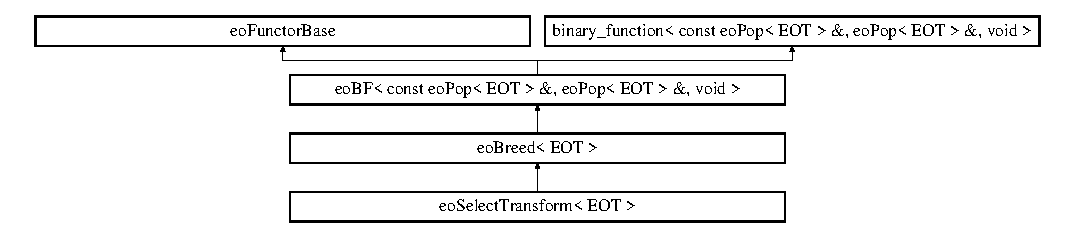
\includegraphics[height=2.75184cm]{classeo_select_transform}
\end{center}
\end{figure}
\subsection*{Public Member Functions}
\begin{CompactItemize}
\item 
{\bf eo\-Select\-Transform} ({\bf eo\-Select}$<$ {\bf EOT} $>$ \&\_\-select, {\bf eo\-Transform}$<$ {\bf EOT} $>$ \&\_\-transform)\label{classeo_select_transform_a0}

\item 
void {\bf operator()} (const {\bf eo\-Pop}$<$ {\bf EOT} $>$ \&\_\-parents, {\bf eo\-Pop}$<$ {\bf EOT} $>$ \&\_\-offspring)\label{classeo_select_transform_a1}

\begin{CompactList}\small\item\em The pure virtual function that needs to be implemented by the subclass. \item\end{CompactList}\end{CompactItemize}
\subsection*{Private Attributes}
\begin{CompactItemize}
\item 
{\bf eo\-Select}$<$ {\bf EOT} $>$ \& {\bf select}\label{classeo_select_transform_r0}

\item 
{\bf eo\-Transform}$<$ {\bf EOT} $>$ \& {\bf transform}\label{classeo_select_transform_r1}

\end{CompactItemize}


\subsection{Detailed Description}
\subsubsection*{template$<$class EOT$>$ class eo\-Select\-Transform$<$ EOT $>$}

Embedded select, followed by an embedded transform. 

Special breeder that is just an application of an embedded select, followed by an embedded transform 



Definition at line 57 of file eo\-Breed.h.

The documentation for this class was generated from the following file:\begin{CompactItemize}
\item 
eo\-Breed.h\end{CompactItemize}
